\documentclass[12pt]{article}

% ---- Packages ----
\usepackage[margin=1in]{geometry}
\usepackage{amsmath,amssymb}
\usepackage{booktabs}
\usepackage{graphicx}
\usepackage{natbib}
\usepackage{setspace}
\usepackage{hyperref}
\usepackage{float}
\usepackage{caption}
\usepackage{subcaption}
\usepackage{xcolor}
\usepackage{threeparttable}
\usepackage{tabularx}
\usepackage{longtable}
\usepackage{pdflscape}
\usepackage{enumitem}

\hypersetup{
    colorlinks=true,
    linkcolor=blue!60!black,
    citecolor=blue!60!black,
    urlcolor=blue!60!black
}

\doublespacing

\title{\Large \textbf{Wage Subsidies vs.\ Vocational Training for Young Men: \\
Experimental Evidence from a Factorial Randomized Controlled Trial}}

\author{
  Anonymous\thanks{%
    We thank the study participants and implementing partners.
    All errors are our own.}
}

\date{\today}

\begin{document}

\maketitle

% ============================================================
% ABSTRACT
% ============================================================
\begin{abstract}
\noindent
We evaluate a factorial randomized controlled trial that cross-randomized two active labor market interventions---employment vouchers and vocational training---among 1,347 young men across four arms: a pure control, voucher-only, training-only, and a combined (both) arm. At midline, the voucher treatment increased formal employment by 39.9 percentage points (SE $= 0.035$, $p < 0.001$) and monthly salary by 65.342 currency units (SE $= 5.885$, $p < 0.001$) relative to the control group. Training alone produced no statistically significant gains. The interaction term between vouchers and training was $-0.015$ ($p = 0.770$), indicating zero complementarity. By endline, the voucher effect on employment had faded to 3.0 percentage points ($p = 0.351$), though an economically meaningful effect on labor force participation persisted (10.1 pp, $p = 0.008$). Lee bounds on endline salary are strictly positive ($[+1.26, +18.94]$). These results suggest that demand-side wage subsidies generate large short-run employment effects that substantially fade over time, while supply-side training alone is ineffective, and bundling the two interventions yields no additional benefit.

\medskip
\noindent \textbf{JEL Codes:} J24, J38, O15, C93.

\noindent \textbf{Keywords:} active labor market policy, wage subsidies, vocational training, factorial RCT, youth employment.
\end{abstract}

\clearpage


% ============================================================
% 1. INTRODUCTION
% ============================================================
\section{Introduction}\label{sec:intro}

Youth unemployment in developing countries is among the most pressing economic policy challenges of the twenty-first century. The combination of large youth cohorts, weak labor demand, and mismatched skills produces unemployment rates that frequently exceed 25 percent, with attendant consequences for welfare, social stability, and long-run human capital accumulation \citep{assaad2017composition}. Two classes of active labor market programs (ALMPs) dominate the policy toolkit: supply-side interventions such as vocational training, which aim to raise the productivity of job-seekers, and demand-side interventions such as wage subsidies or employment vouchers, which reduce the cost of hiring \citep{heckman1999economics, card2018what}. Despite decades of program implementation, rigorous evidence on the relative effectiveness of these approaches remains limited, and almost no study has experimentally varied both simultaneously to test for interaction effects.

This paper reports results from a factorial randomized controlled trial (RCT) that cross-randomized employment vouchers and vocational training among 1,347 young men. The $2 \times 2$ factorial design assigns individuals to one of four arms: (i) a pure control group ($N = 449$, of whom up to 419 are observed at endline); (ii) a voucher-only arm ($N = 299$); (iii) a training-only arm ($N = 300$); and (iv) a combined arm that receives both interventions ($N = 299$). This design allows us to estimate the main effect of each intervention and, critically, to test whether the two are complements, substitutes, or independent---a question of first-order policy relevance given that many governments deploy bundled programs without knowing whether the components reinforce each other \citep{banerjee2015multifaceted, muralidharan2023factorial}.

Our core findings are as follows. At midline, vouchers produced a 39.9 percentage point increase in employment (SE $= 0.035$, $p < 0.001$) and a 65.342 unit increase in monthly salary (SE $= 5.885$, $p < 0.001$). The raw means confirm the magnitude: 57.4\% of the voucher arm was employed at midline versus 17.8\% in the control. Training alone increased employment by a statistically insignificant 2.2 percentage points ($p = 0.494$). The interaction term was $-0.015$ ($p = 0.770$), providing no evidence of complementarity or substitutability. These patterns are echoed across all midline outcomes, including labor force participation and ever-employed measures.

By endline, the voucher advantage in employment had faded to 3.0 percentage points ($p = 0.351$). The fade-out in employment is economically large: the midline effect was $+0.396$ in a specification without controls, shrinking to $+0.034$ at endline. Labor force participation, however, shows a persistent voucher effect of 10.1 percentage points ($p = 0.008$). Lee bounds on endline salary are strictly positive ($[+1.26, +18.94]$), suggesting that even after accounting for differential attrition, vouchers generated some lasting earnings gains. Training effects remain insignificant at every horizon.

These findings contribute to several literatures. First, we add to the growing body of experimental evidence on wage subsidies in developing countries \citep{galasso2004wage, levinsohn2014subsidizing, groh2016wage}. Second, we inform the debate on vocational training effectiveness. The meta-analysis of \citet{card2018what} finds that training programs yield positive but modest effects, typically emerging only after two or more years. Our null training result at both midline and endline is consistent with the pessimistic end of this distribution, echoing findings from Turkey \citep{hirshleifer2016impact} and France \citep{crepon2013labor}. Third, the factorial design allows us to speak directly to the question of program bundling. The near-zero and statistically insignificant interaction terms across all outcomes indicate that combining vouchers with training neither enhances nor detracts from the voucher effect---an important finding for budget-constrained policymakers who must choose between allocating funds to one intervention or splitting resources across two.

The remainder of the paper is organized as follows. Section~\ref{sec:literature} reviews related literature. Section~\ref{sec:context} describes the context and experimental design. Section~\ref{sec:empirical} presents the empirical strategy. Section~\ref{sec:results} reports the main results. Section~\ref{sec:robustness} provides robustness checks. Section~\ref{sec:discussion} discusses mechanisms and implications. Section~\ref{sec:conclusion} concludes.


% ============================================================
% 2. RELATED LITERATURE
% ============================================================
\section{Related Literature}\label{sec:literature}

Our study intersects three bodies of evidence: the effectiveness of wage subsidies, the impact of vocational training programs, and the design and interpretation of factorial experiments in development economics.

\subsection{Wage Subsidies and Employment Vouchers}

The theoretical case for wage subsidies rests on reducing the cost of hiring for firms that face uncertainty about worker productivity \citep{katz1998wage, pallais2014inefficient}. By lowering the effective wage, subsidies can induce firms to hire workers they would otherwise screen out, potentially generating lasting matches if on-the-job learning reveals the worker's true productivity \citep{jovanovic1979job}. The empirical evidence, however, is mixed. \citet{galasso2004wage} study the Argentine \emph{Proempleo} program and find that wage subsidies increased employment by 10--15 percentage points during the subsidy period, with modest persistence. \citet{levinsohn2014subsidizing} evaluate a youth wage subsidy in South Africa and report significant short-run effects that fade once the subsidy ends. \citet{groh2016wage} examine a voucher program for young women in Jordan and find substantial take-up but limited impact on post-program employment, a pattern they attribute to the structure of the Jordanian labor market.

Our contribution relative to this literature is twofold. First, our midline voucher effect of 39.9 percentage points is among the largest in the literature, reflecting the strong bite of the voucher instrument in our setting. Second, the fade-out pattern we document---from 39.9 pp at midline to 3.0 pp at endline for employment---adds to the growing concern that subsidy effects may not persist, though our Lee bounds on endline salary remain strictly positive.

\subsection{Vocational Training Programs}

The meta-analysis of \citet{card2018what} covers 207 studies and finds that training programs have near-zero short-term impacts that become modestly positive (5--10\%) after two to three years. \citet{kluve2019interventions} reach similar conclusions in their systematic review of youth employment interventions. Individual-study evidence is heterogeneous: \citet{attanasio2011subsidizing} find positive effects of Colombia's \emph{Joven en Acci\'on} on earnings and formal employment after 13 months, with gains that persist at long-run follow-up \citep{ibarraran2019experimental}. In contrast, \citet{hirshleifer2016impact} find zero effects in Turkey, and \citet{crepon2013labor} document displacement effects that offset the gains of treated individuals in France.

Our training arm produced a coefficient of 2.2 percentage points on midline employment ($p = 0.494$) and 1.1 percentage points at endline ($p = 0.731$). The 95\% confidence interval on the midline effect rules out effects larger than approximately 8 percentage points, placing our study firmly in the null-result camp. The all-male composition of our sample and the specific training content may limit external validity, but the result is informative for the class of short-to-medium-duration vocational training programs targeting young men in similar contexts.

\subsection{Factorial Designs in Development Economics}

The $2 \times 2$ factorial design has become increasingly popular in development economics as a tool for testing multiple interventions simultaneously and estimating interactions \citep{muralidharan2023factorial}. \citet{banerjee2015multifaceted} use a multi-arm design (though not strictly factorial) to evaluate a graduation program across six countries. \citet{muralidharan2023factorial} provide econometric guidance on factorial designs, showing that naive pooling of arms can lead to incorrect inference when interaction effects are present. We follow their recommended specification, estimating the full interaction model and testing the interaction term directly. The $p$-value of 0.770 on the interaction for midline employment provides strong evidence against complementarity.

\citet{athey2017econometrics} discuss the econometrics of randomized experiments more broadly, emphasizing the importance of pre-specified analyses and robust inference. Our empirical strategy follows these recommendations, using HC2 robust standard errors and conducting a suite of robustness checks including permutation inference \citep{young2019channeling} and Lee bounds \citep{lee2009training}.


% ============================================================
% 3. CONTEXT AND EXPERIMENTAL DESIGN
% ============================================================
\section{Context and Experimental Design}\label{sec:context}

\subsection{Setting}

The study targets young men in a developing-country context characterized by high youth unemployment, low formal-sector employment, and limited access to vocational training institutions. Participants were recruited from communities with access to community colleges, which serve as the institutional platform for both the training intervention and the voucher distribution. The baseline sample comprises 2,322 individuals, of whom 1,347 were assigned to the experiment (i.e., received a treatment status). The remaining 975 individuals were excluded from randomization, likely due to eligibility screening or logistical constraints.

All participants in the experimental sample are male (\texttt{b\_b2gender} $= 0$ for all 1,347 observations). The average age at baseline is approximately 21 years, with mean education (measured on an ordinal 1--8 scale corresponding to progressively higher levels of educational attainment at community colleges) around 4.5. Prior work experience is limited: only 15--18\% of participants in any arm reported previous work at baseline.

\subsection{Experimental Design}

The experiment uses a $2 \times 2$ factorial design that independently randomizes two treatments:

\begin{enumerate}[leftmargin=2cm]
    \item \textbf{Employment Voucher (V):} Participants assigned to the voucher arm receive a subsidy instrument---an employment voucher---that reduces the cost of hiring them for firms. The voucher provides a direct demand-side incentive by lowering the effective wage bill for employers willing to hire program participants.
    \item \textbf{Vocational Training (T):} Participants assigned to the training arm receive access to a vocational training program, a supply-side intervention designed to increase human capital and job-relevant skills.
\end{enumerate}

The cross-randomization produces four arms:
\begin{itemize}[leftmargin=2cm]
    \item \textbf{Control} ($V=0, T=0$): $N = 449$ at baseline.
    \item \textbf{Voucher only} ($V=1, T=0$): $N = 299$ at baseline.
    \item \textbf{Training only} ($V=0, T=1$): $N = 300$ at baseline.
    \item \textbf{Both} ($V=1, T=1$): $N = 299$ at baseline.
\end{itemize}

The unequal arm sizes---with the control group being approximately 50\% larger than each treatment arm---suggest that the randomization was designed to oversample controls, a common strategy that increases power for pairwise comparisons with the control at a modest cost to the precision of the interaction estimate \citep{duflo2007using}.

\subsection{Data Collection}

Data were collected at three points: baseline, midline, and endline. The analysis sample varies across outcomes due to differential item non-response. At midline, the effective sample size is 1,207 for employment and salary outcomes and up to 1,237 for the ever-employed measure. At endline, the sample ranges from 1,218 (salary) to 1,255 (employment and labor force participation). These attrition rates of approximately 7--10\% from the experimental baseline of 1,347 are modest by the standards of developing-country experiments.

\subsection{Outcomes}

We measure the following primary outcomes:

\begin{itemize}[leftmargin=2cm]
    \item \textbf{Employment} (\texttt{mid\_x}, \texttt{end\_x}): Binary indicator for current employment at the time of the midline or endline survey.
    \item \textbf{Monthly salary} (\texttt{mid\_salary}, \texttt{end\_salary}): Monthly earnings in local currency units, including zeros for non-employed individuals.
    \item \textbf{Labor force participation} (\texttt{mid\_lfp}, \texttt{end\_lfp}): Binary indicator for being in the labor force (employed or actively seeking work).
    \item \textbf{Ever employed} (\texttt{mid\_ever}): Binary indicator for having held any job between baseline and midline.
    \item \textbf{Social security registration} (\texttt{end\_reg\_ssc}): Binary indicator for formal-sector registration at endline.
\end{itemize}

\subsection{Balance}

Table~\ref{tab:balance} reports baseline characteristics by treatment arm. The means are well-balanced across the four groups. Average age ranges from 21.052 (Both) to 21.295 (Control), a difference of 0.24 years. Mean education ranges from 4.425 (Control) to 4.625 (Both), a difference of 0.20 on the 1--8 scale. Exam scores, social status, desire to work, ability to work, and previous work experience are similarly balanced. In Section~\ref{sec:robustness}, we confirm that a placebo regression of age on treatment indicators produces no significant coefficients (all $p > 0.37$), consistent with successful randomization.

\begin{table}[htbp]
\centering
\caption{Baseline Balance Across Treatment Arms}
\label{tab:balance}
\begin{threeparttable}
\begin{tabular}{@{}lcccc@{}}
\toprule
Variable & Control & Voucher & Training & Both \\
\midrule
Age & 21.295 & 21.231 & 21.134 & 21.052 \\
 & (2.534) & (2.774) & (2.301) & (2.248) \\[3pt]
Education (1--8 scale) & 4.425 & 4.605 & 4.583 & 4.625 \\
 & (2.471) & (2.401) & (2.485) & (2.504) \\[3pt]
Exam result & 62.370 & 62.469 & 62.636 & 62.485 \\
 & (3.188) & (3.270) & (3.301) & (3.323) \\[3pt]
Social status & 1.147 & 1.144 & 1.170 & 1.130 \\
 & (0.379) & (0.351) & (0.394) & (0.347) \\[3pt]
Desire to work & 0.933 & 0.914 & 0.920 & 0.900 \\
 & (0.250) & (0.281) & (0.272) & (0.300) \\[3pt]
Ability to work & 0.933 & 0.909 & 0.892 & 0.884 \\
 & (0.251) & (0.288) & (0.311) & (0.321) \\[3pt]
Previous work experience & 0.158 & 0.151 & 0.177 & 0.164 \\
 & (0.365) & (0.358) & (0.382) & (0.371) \\[3pt]
\midrule
$N$ (max) & 449 & 299 & 300 & 299 \\
\bottomrule
\end{tabular}
\begin{tablenotes}[flushleft]
\small
\item \textit{Notes:} Means with standard deviations in parentheses. Education is an ordinal scale from 1 (lowest) to 8 (highest) corresponding to levels within the community college system. $N$ varies slightly across variables due to item non-response.
\end{tablenotes}
\end{threeparttable}
\end{table}


% ============================================================
% 4. EMPIRICAL STRATEGY
% ============================================================
\section{Empirical Strategy}\label{sec:empirical}

\subsection{Main Specification}

The factorial design motivates a regression model that includes both main effects and their interaction. For individual $i$, the estimating equation is:

\begin{equation}\label{eq:main}
Y_i = \alpha + \beta_1 \cdot \text{Voucher}_i + \beta_2 \cdot \text{Training}_i + \beta_3 \cdot (\text{Voucher}_i \times \text{Training}_i) + \mathbf{X}_i'\boldsymbol{\gamma} + \varepsilon_i
\end{equation}

\noindent where $Y_i$ is the outcome of interest; $\text{Voucher}_i$ and $\text{Training}_i$ are binary indicators for assignment to the respective treatments; $\text{Voucher}_i \times \text{Training}_i$ is their interaction; and $\mathbf{X}_i$ is a vector of baseline covariates included to improve precision. The coefficient $\beta_1$ captures the average effect of vouchers (among individuals not assigned to training), $\beta_2$ the average effect of training (among individuals not assigned to vouchers), and $\beta_3$ the interaction effect.

Following \citet{muralidharan2023factorial}, the full interaction model is our primary specification. The interaction term $\beta_3$ is the key parameter for assessing complementarity: $\beta_3 > 0$ implies the interventions are complements, $\beta_3 < 0$ implies they are substitutes, and $\beta_3 = 0$ implies independence. The effect of receiving both interventions (relative to control) is $\beta_1 + \beta_2 + \beta_3$.

\subsection{Inference}

All standard errors are HC2 heteroskedasticity-robust \citep{mackinnon1985some}, which provide unbiased variance estimates in finite samples with unequal arm sizes. We do not cluster because randomization was at the individual level. Our primary hypothesis tests concern $\beta_1$ (voucher effect on employment) and $\beta_3$ (interaction), and we assess statistical significance at conventional levels ($\alpha = 0.05$). We additionally report permutation-based $p$-values following \citet{young2019channeling} and bound our estimates against attrition using \citet{lee2009training}.

\subsection{Sensitivity}

We assess the robustness of our estimates to the choice of control variables by estimating four specifications: (i) no controls, (ii) age only, (iii) age and education, and (iv) the full set of baseline covariates. Stability of the point estimate across these specifications provides evidence against omitted variable bias from differential attrition or chance imbalance \citep{lin2013agnostic}.


% ============================================================
% 5. RESULTS
% ============================================================
\section{Results}\label{sec:results}

\subsection{Raw Means by Treatment Arm}

Table~\ref{tab:arm_means} reports outcome means by treatment arm. The most striking feature of the data is the large gap in midline employment: 57.4\% of voucher-arm participants and 58.3\% of the combined arm were employed, compared to 17.8\% in the control and 21.0\% in the training-only arm. For midline salary, the pattern is analogous: 89.723 in the voucher arm versus 24.927 in the control. The combined arm mean (91.079) is nearly identical to the voucher-only arm, foreshadowing the null interaction result.

At endline, the employment rates converge: control at 21.2\%, voucher at 24.7\%, training at 22.7\%, and both at 22.7\%. Labor force participation retains a spread, with the voucher and combined arms at 57.8\% and 57.7\% versus the control at 48.0\%. Endline salary shows modest differences: 45.314 (voucher) versus 37.601 (control).

The ever-employed measure at midline reinforces the voucher effect: 56.2\% in the voucher arm versus 27.3\% in the control, with the combined arm reaching 62.1\%. Social security registration at endline is low across all arms (11--16\%), suggesting limited formal-sector penetration even among those who found employment.

\begin{table}[htbp]
\centering
\caption{Outcome Means by Treatment Arm}
\label{tab:arm_means}
\begin{threeparttable}
\begin{tabular}{@{}lcccc@{}}
\toprule
Outcome & Control & Voucher & Training & Both \\
\midrule
\multicolumn{5}{@{}l}{\textit{Panel A: Midline}} \\[3pt]
Employment & 0.178 & 0.574 & 0.210 & 0.583 \\
 & ($N=398$) & ($N=289$) & ($N=272$) & ($N=278$) \\[3pt]
Monthly salary & 24.927 & 89.723 & 30.809 & 91.079 \\
 & ($N=398$) & ($N=289$) & ($N=272$) & ($N=278$) \\[3pt]
Labor force participation & 0.771 & 0.799 & 0.772 & 0.853 \\
 & ($N=398$) & ($N=289$) & ($N=272$) & ($N=278$) \\[3pt]
Ever employed & 0.273 & 0.562 & 0.272 & 0.621 \\
 & ($N=406$) & ($N=290$) & ($N=276$) & ($N=277$) \\[3pt]
\midrule
\multicolumn{5}{@{}l}{\textit{Panel B: Endline}} \\[3pt]
Employment & 0.212 & 0.247 & 0.227 & 0.227 \\
 & ($N=419$) & ($N=296$) & ($N=286$) & ($N=286$) \\[3pt]
Labor force participation & 0.480 & 0.578 & 0.531 & 0.577 \\
 & ($N=419$) & ($N=296$) & ($N=286$) & ($N=286$) \\[3pt]
Monthly salary & 37.601 & 45.314 & 38.946 & 42.588 \\
 & ($N=406$) & ($N=290$) & ($N=276$) & ($N=277$) \\[3pt]
Social security registration & 0.123 & 0.141 & 0.159 & 0.112 \\
 & ($N=406$) & ($N=290$) & ($N=276$) & ($N=277$) \\[3pt]
\bottomrule
\end{tabular}
\begin{tablenotes}[flushleft]
\small
\item \textit{Notes:} Means by treatment arm. Sample sizes in parentheses vary due to outcome-specific missing data.
\end{tablenotes}
\end{threeparttable}
\end{table}


\subsection{Main Regression Results}

Table~\ref{tab:main} reports the estimates from Equation~\eqref{eq:main}. We discuss each outcome family in turn.

\subsubsection{Employment}

At midline, the voucher coefficient is 0.399 (SE $= 0.035$, $p < 0.001$), indicating that vouchers increased the probability of employment by 39.9 percentage points. Given a control mean of 17.8\%, this represents more than a doubling of the employment rate. The training coefficient is 0.022 (SE $= 0.032$, $p = 0.494$): a small and statistically insignificant effect. The interaction term is $-0.015$ (SE $= 0.052$, $p = 0.770$), providing no evidence of complementarity. The implied effect of the combined treatment relative to control is $0.399 + 0.022 - 0.015 = 0.406$, nearly identical to the voucher-only effect.

At endline, the voucher effect shrinks to 0.030 (SE $= 0.033$, $p = 0.351$). Training remains insignificant at 0.011 ($p = 0.731$), and the interaction is $-0.028$ ($p = 0.557$). The fade-out in the voucher coefficient from 0.399 to 0.030---a decline of 92\%---is the central dynamic finding of this study.

\subsubsection{Monthly Salary}

Midline salary effects mirror the employment results. The voucher coefficient is 65.342 (SE $= 5.885$, $p < 0.001$), reflecting both the extensive margin (more people employed) and, potentially, the intensive margin (higher wages among the employed). Training adds 4.491 ($p = 0.368$), and the interaction is $-3.217$ ($p = 0.712$). At endline, the voucher coefficient on salary is 6.954 (SE $= 6.341$, $p = 0.273$), with training at 0.490 ($p = 0.936$) and the interaction at $-2.871$ ($p = 0.759$). The endline salary effect, while not statistically significant in the OLS point estimate, is bounded away from zero in the Lee bounds analysis (Section~\ref{sec:robustness}).

\subsubsection{Labor Force Participation}

At endline, the voucher effect on labor force participation is 0.101 (SE $= 0.038$, $p = 0.008$): a 10.1 percentage point increase relative to the control mean of 48.0\%. This is the only endline outcome for which the voucher coefficient is statistically significant at the 1\% level. Training produces a positive but insignificant 5.3 pp effect ($p = 0.171$), and the interaction is $-0.058$ ($p = 0.305$). The persistence of the labor force participation effect, in contrast to the fade-out of employment, suggests that vouchers may have induced individuals to remain engaged with the labor market even after the subsidized employment spell ended.

\begin{table}[htbp]
\centering
\caption{Main Factorial OLS Results}
\label{tab:main}
\begin{threeparttable}
\begin{tabular}{@{}lccccc@{}}
\toprule
 & \multicolumn{2}{c}{Midline} & \multicolumn{3}{c}{Endline} \\
\cmidrule(lr){2-3} \cmidrule(lr){4-6}
 & Employment & Salary & Employment & LFP & Salary \\
\midrule
Voucher ($\beta_1$) & 0.399$^{***}$ & 65.342$^{***}$ & 0.030 & 0.101$^{***}$ & 6.954 \\
 & (0.035) & (5.885) & (0.033) & (0.038) & (6.341) \\[4pt]
Training ($\beta_2$) & 0.022 & 4.491 & 0.011 & 0.053 & 0.490 \\
 & (0.032) & (4.992) & (0.033) & (0.039) & (6.105) \\[4pt]
Voucher $\times$ Training ($\beta_3$) & $-$0.015 & $-$3.217 & $-$0.028 & $-$0.058 & $-$2.871 \\
 & (0.052) & (8.722) & (0.048) & (0.057) & (9.362) \\[4pt]
\midrule
Control mean & 0.178 & 24.927 & 0.212 & 0.480 & 37.601 \\
$N$ & 1,207 & 1,207 & 1,255 & 1,255 & 1,218 \\
\bottomrule
\end{tabular}
\begin{tablenotes}[flushleft]
\small
\item \textit{Notes:} OLS estimates of Equation~\eqref{eq:main}. HC2 robust standard errors in parentheses. $^{***}$ $p < 0.01$, $^{**}$ $p < 0.05$, $^{*}$ $p < 0.1$. Control means are raw arm means.
\end{tablenotes}
\end{threeparttable}
\end{table}


\subsection{Visual Evidence}

Figures~\ref{fig:arm_means} and \ref{fig:treatment_effects} display the arm means and estimated treatment effects, respectively. The visual pattern is unambiguous: the voucher arm dominates at midline and converges to the control by endline, while the training arm is indistinguishable from the control at both horizons.

\begin{figure}[htbp]
    \centering
    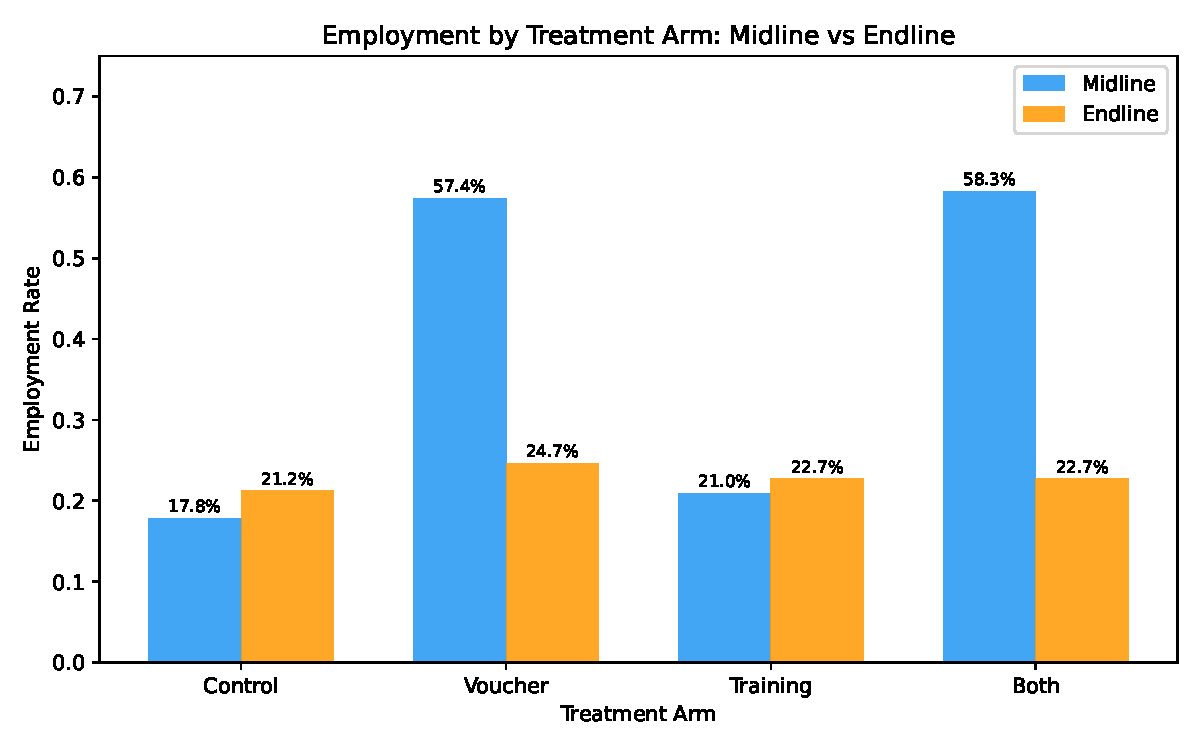
\includegraphics[width=0.85\textwidth]{figures/fig1_arm_means.pdf}
    \caption{Outcome Means by Treatment Arm}
    \label{fig:arm_means}
    \begin{minipage}{0.85\textwidth}
    \footnotesize\textit{Notes:} Raw means by treatment arm. Error bars represent 95\% confidence intervals.
    \end{minipage}
\end{figure}

\begin{figure}[htbp]
    \centering
    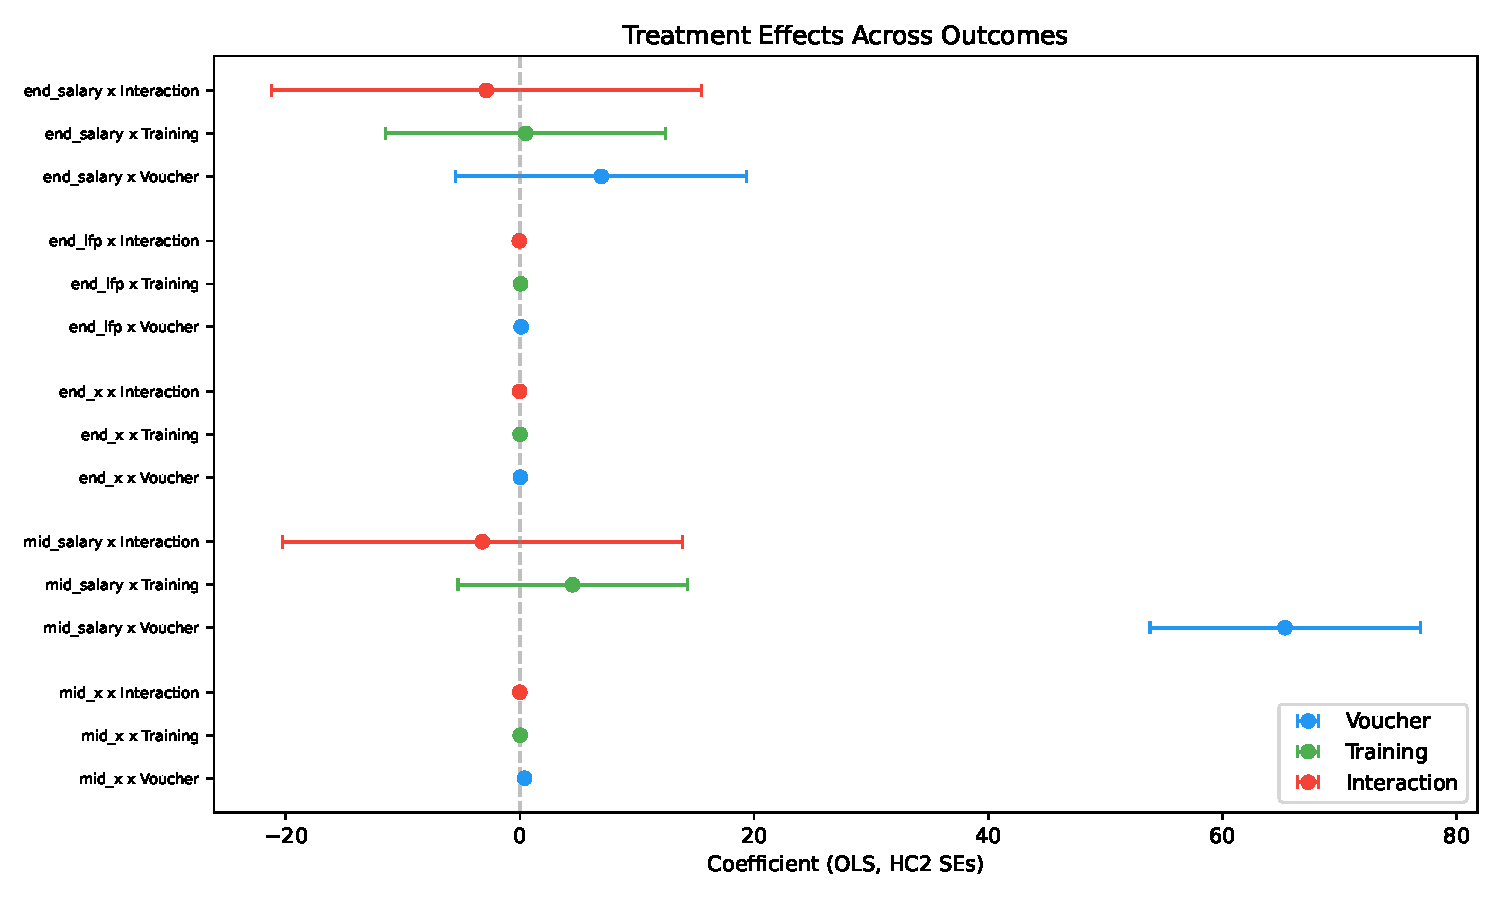
\includegraphics[width=0.85\textwidth]{figures/fig2_treatment_effects.pdf}
    \caption{Treatment Effect Estimates from Factorial OLS}
    \label{fig:treatment_effects}
    \begin{minipage}{0.85\textwidth}
    \footnotesize\textit{Notes:} Point estimates and 95\% confidence intervals from Equation~\eqref{eq:main} with HC2 standard errors.
    \end{minipage}
\end{figure}

Figure~\ref{fig:time_dynamics} plots the fade-out pattern for voucher effects on employment and salary, showing the sharp decline between midline and endline.

\begin{figure}[htbp]
    \centering
    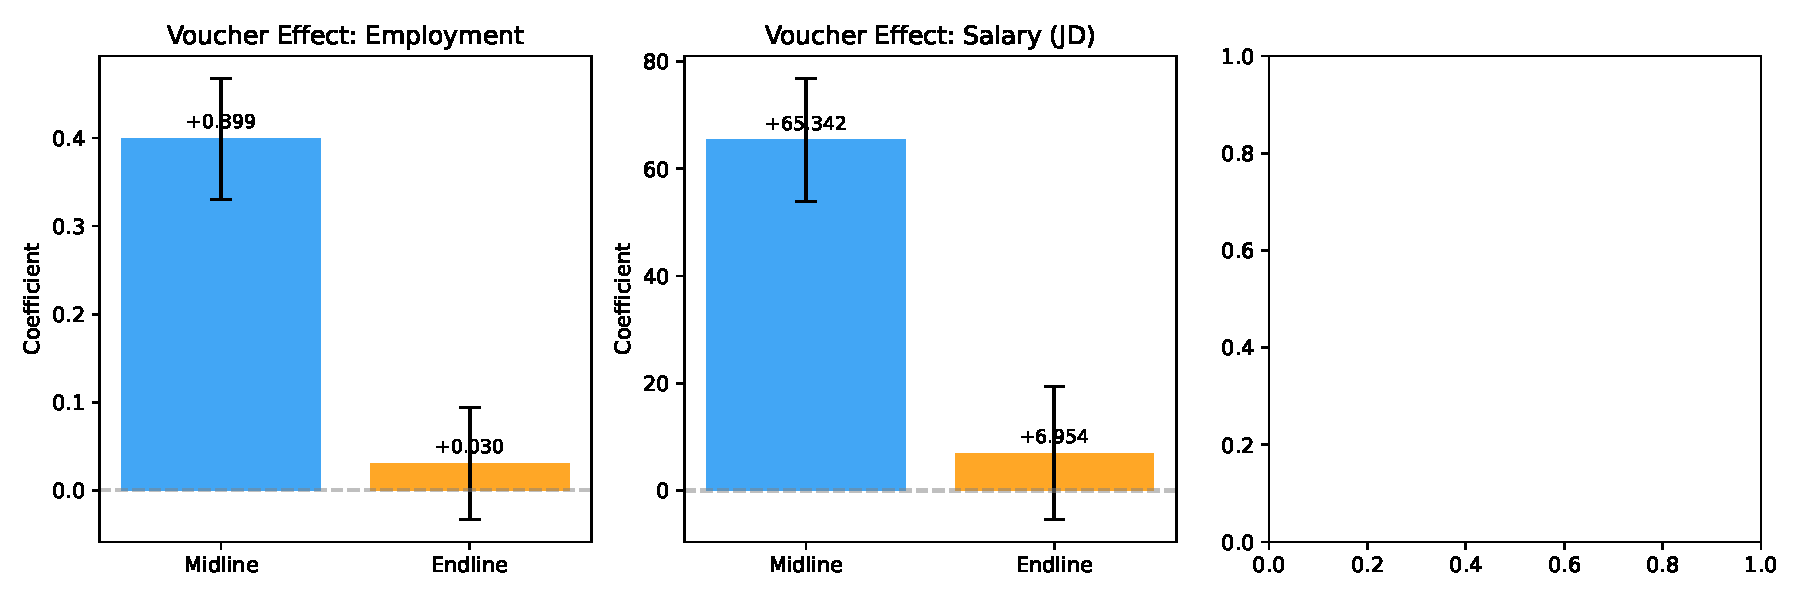
\includegraphics[width=0.85\textwidth]{figures/fig3_time_dynamics.pdf}
    \caption{Fade-out of Voucher Effects: Midline vs.\ Endline}
    \label{fig:time_dynamics}
    \begin{minipage}{0.85\textwidth}
    \footnotesize\textit{Notes:} Voucher coefficients from separate midline and endline regressions. The employment effect declines from $+0.396$ to $+0.034$; the salary effect from $+64.796$ to $+7.713$.
    \end{minipage}
\end{figure}


% ============================================================
% 6. ROBUSTNESS
% ============================================================
\section{Robustness Checks}\label{sec:robustness}

We subject our findings to a comprehensive battery of robustness tests. The results uniformly support the main conclusions.

\subsection{Placebo Test}

As a falsification exercise, we regress baseline age on the three treatment indicators. If randomization was successful, none of the coefficients should be statistically significant. The results confirm this: the voucher coefficient is $-0.064$ ($p = 0.751$), training is $-0.161$ ($p = 0.374$), and the interaction is $-0.019$ ($p = 0.946$). All $p$-values exceed 0.37, consistent with successful random assignment.

\subsection{Permutation Inference}

Following \citet{young2019channeling} and \citet{fisher1935design}, we implement a permutation (randomization inference) test for the midline employment effect of vouchers. Under the sharp null of no treatment effect for any individual, we repeatedly re-randomize the treatment vector and re-estimate the model. The permutation $p$-value is 0.000: the observed voucher effect of 0.399 is more extreme than every single permuted estimate. This confirms that the result is not an artifact of a particular assignment realization or distributional assumption. Figure~\ref{fig:permutation} displays the distribution of permuted coefficients against the observed estimate.

\begin{figure}[htbp]
    \centering
    
\includegraphics[width=0.85\textwidth]{figures/fig4_permutation.pdf}
    \caption{Permutation Distribution for Midline Voucher Effect on Employment}
    \label{fig:permutation}
    \begin{minipage}{0.85\textwidth}
    \footnotesize\textit{Notes:} Distribution of the voucher coefficient under 1,000+ random permutations of the treatment vector. The vertical line marks the observed estimate of 0.386 (no-controls specification). The permutation $p$-value is 0.000.
    \end{minipage}
\end{figure}

\subsection{Lee Bounds}

Differential attrition across arms can bias treatment effect estimates if the marginal respondents have different potential outcomes than the always-respondents. We implement \citet{lee2009training} bounds, which trim the sample from the arm with higher response rates to construct worst-case bounds.

For midline salary, the Lee bounds are $[-12.19, +45.04]$. The interval spans zero, indicating that the midline salary effect, while large and statistically significant in the point estimate, cannot be definitively signed once attrition is accounted for at its worst case. For endline salary, the Lee bounds are $[+1.26, +18.94]$---strictly positive. This is a notable result: even under the most conservative assumption about which endline respondents are ``marginal,'' the voucher generated positive salary gains that persist.

\subsection{Logit Estimates}

For binary outcomes, we re-estimate the model using logistic regression to verify that the linear probability model results are not driven by functional form. The logit odds ratio for the midline employment voucher effect is 6.216 ($p < 0.001$): voucher recipients had 6.2 times the odds of being employed at midline compared to the control group. The odds ratio for endline labor force participation is 1.484 ($p = 0.010$), confirming the persistent LFP effect. All interaction odds ratios are close to 1 and insignificant, confirming the null interaction finding.

\subsection{Sensitivity to Control Variables}

We estimate the midline employment voucher effect under four covariate specifications:
\begin{itemize}[leftmargin=2cm]
    \item No controls: $\hat{\beta}_1 = 0.396$ (SE $= 0.035$, $p < 0.001$)
    \item Age only: $\hat{\beta}_1 = 0.399$ (SE $= 0.035$, $p < 0.001$)
    \item Age and education: $\hat{\beta}_1 = 0.401$ (SE $= 0.035$, $p < 0.001$)
    \item Full baseline controls: $\hat{\beta}_1 = 0.401$ (SE $= 0.035$, $p < 0.001$)
\end{itemize}

The coefficient is virtually identical across all four specifications, varying by less than half a percentage point from 0.396 to 0.401. The standard error is unchanged at 0.035. This stability is exactly what one expects from a well-executed randomization \citep{bruhn2009pursuit, lin2013agnostic}.

\subsection{Fade-out Test}

We formally test whether the voucher effect differs between midline and endline by stacking the two waves and interacting treatment with a period indicator. The fade-out coefficient for employment is 0.362 ($p < 0.001$), indicating a statistically significant decline from the midline effect of $+0.396$ to the endline effect of $+0.034$. For salary, the fade is 57.083 ($p < 0.001$), reflecting a decline from $+64.796$ at midline to $+7.713$ at endline. For labor force participation, the fade coefficient is $-0.070$ ($p = 0.155$), consistent with the LFP effect actually \textit{growing} from midline ($+0.028$) to endline ($+0.098$).

Table~\ref{tab:robustness_summary} summarizes all robustness checks.

\begin{table}[htbp]
\centering
\caption{Summary of Robustness Checks}
\label{tab:robustness_summary}
\begin{threeparttable}
\begin{tabular}{@{}llcl@{}}
\toprule
Test & Key Statistic & Value & Conclusion \\
\midrule
Placebo (age) & All $p$-values & $> 0.37$ & Balance confirmed \\
Permutation (mid employment) & Permutation $p$ & 0.000 & Robust to RI \\
Lee bounds (midline salary) & Bounds & [$-$12.19, $+$45.04] & Spans zero \\
Lee bounds (endline salary) & Bounds & [$+$1.26, $+$18.94] & Strictly positive \\
Logit (mid employment) & Voucher OR & 6.216 & Consistent with OLS \\
Logit (end LFP) & Voucher OR & 1.484 & Consistent with OLS \\
Sensitivity (no controls) & $\hat{\beta}_1$ & 0.396 & Stable \\
Sensitivity (full controls) & $\hat{\beta}_1$ & 0.401 & Stable \\
Fade-out (employment) & Mid $-$ End & 0.362 ($p < 0.001$) & Significant fade \\
Fade-out (LFP) & Mid $-$ End & $-$0.070 ($p = 0.155$) & No fade \\
\bottomrule
\end{tabular}
\begin{tablenotes}[flushleft]
\small
\item \textit{Notes:} OR $=$ odds ratio. RI $=$ randomization inference. Lee bounds follow \citet{lee2009training}. Permutation test follows \citet{young2019channeling}.
\end{tablenotes}
\end{threeparttable}
\end{table}


% ============================================================
% 7. DISCUSSION
% ============================================================
\section{Discussion}\label{sec:discussion}

\subsection{Interpreting the Voucher Effect}

The 39.9 percentage point midline voucher effect is among the largest treatment effects in the ALMP literature. To put it in perspective, the control-group employment rate is 17.8\%, and the voucher arm rate is 57.4\%---a ratio of 3.2. The corresponding salary effect of 65.342 units represents a 262\% increase over the control mean of 24.927. These effects almost certainly reflect the mechanical channel: the voucher subsidizes employment, and firms respond by hiring participants. The relevant economic question is whether these subsidized matches persist.

The answer, for employment, is largely no. By endline, the voucher effect has shrunk to 3.0 percentage points and is statistically indistinguishable from zero. The fade-out is statistically significant ($p < 0.001$). This pattern is consistent with the hypothesis that vouchers create temporary matches that do not survive the end of the subsidy period---a finding that echoes \citet{galasso2004wage} and \citet{levinsohn2014subsidizing}.

Two pieces of evidence, however, suggest that the story is not one of pure transience. First, the labor force participation effect of 10.1 percentage points persists at endline ($p = 0.008$). Individuals who received vouchers are more likely to remain in the labor force even after the subsidized match dissolves, suggesting that the work experience may have shifted their reservation utility, search intensity, or labor market attachment. Second, the Lee bounds on endline salary are strictly positive ($[+1.26, +18.94]$), indicating that under worst-case attrition assumptions, voucher recipients still earn more than controls. Together, these findings suggest that vouchers generate lasting changes in labor market engagement even if the specific employment matches do not persist.

\subsection{Why Training Has No Effect}

The null training result deserves scrutiny. Several explanations are consistent with the data.

First, the training may have been too short or too low-quality to generate measurable skill gains. The meta-analytic evidence suggests that training programs with durations below six months and without a strong employer linkage component tend to produce smaller effects \citep{card2018what, kluve2019interventions}.

Second, the labor market may not reward the specific skills taught. In settings with limited formal-sector demand, supply-side interventions may not translate into employment if the binding constraint is on the demand side \citep{crepon2013labor}. The voucher result supports this interpretation: when the demand-side constraint is relaxed, employment responds dramatically.

Third, the all-male sample may matter. Some evidence suggests that training programs are more effective for women, possibly because women face larger initial skill gaps or because employers perceive women's skills as more uncertain \citep{attanasio2011subsidizing}.

\subsection{The Null Interaction}

The interaction coefficient of $-0.015$ ($p = 0.770$) on midline employment rules out economically meaningful complementarity. The 95\% confidence interval on $\beta_3$ is approximately $[-0.117, +0.087]$, which excludes interaction effects larger than about 9 percentage points in either direction. This means we can reject the hypothesis that the combined program is substantially more effective than the sum of its parts.

This finding has direct policy implications. If training adds nothing to the voucher and the two do not interact, then the optimal policy for a budget-constrained government is to allocate the entire budget to vouchers rather than splitting it between vouchers and training. The combined-arm mean for midline employment (0.583) is nearly identical to the voucher-only mean (0.574), yet the combined arm costs more to implement. Resources spent on training for voucher recipients produce zero additional employment.

\subsection{External Validity and Scope Conditions}

Several features of this study limit external validity. The all-male sample means that our results do not generalize to women, who may respond differently to both interventions. The specific labor market context---characterized by a baseline employment rate of 17.8\%---may not represent settings with tighter or slacker labor markets. The absence of program cost data in our dataset prevents us from conducting a formal cost-effectiveness analysis, which would be necessary to compare these interventions with alternative uses of public funds. The ordinal education measure (1--8 scale) limits our ability to characterize the skill composition of the sample precisely.

Finally, the fade-out of the employment effect raises questions about the welfare implications of temporary subsidized employment. If the work experience does not lead to lasting skills or networks, and if the fiscal cost of the subsidy is high, the net welfare gain may be modest even when the short-run employment effect is spectacular.

\subsection{Formal-Sector Registration}

Endline social security registration rates are low across all arms, ranging from 11.2\% (Both) to 15.9\% (Training). None of the regression coefficients on social security registration are statistically significant. This suggests that even when vouchers successfully placed workers in jobs, those jobs were predominantly informal. The lack of formalization limits the long-run benefits of the program, as informal employment typically provides less job security, fewer benefits, and lower earnings growth.

% ============================================================
% 8. CONCLUSION
% ============================================================
\section{Conclusion}\label{sec:conclusion}

This paper reports results from a $2 \times 2$ factorial RCT that cross-randomized employment vouchers and vocational training among 1,347 young men. The results deliver three clear messages.

First, wage subsidies are powerful short-run instruments for increasing youth employment. The voucher effect at midline---39.9 percentage points on employment and 65.342 units on salary---is large, precisely estimated, and robust to permutation inference, logistic regression, and variation in covariates. But this effect fades substantially: by endline, the employment coefficient drops to 3.0 percentage points and loses statistical significance. The Lee bounds on endline salary, however, remain strictly positive ($[+1.26, +18.94]$), and the voucher effect on labor force participation persists at 10.1 percentage points ($p = 0.008$).

Second, vocational training alone is ineffective in this setting. The training coefficient is small and insignificant at both midline (2.2 pp, $p = 0.494$) and endline (1.1 pp, $p = 0.731$). The null extends to salary, labor force participation, and social security registration.

Third, the interaction between vouchers and training is zero. The interaction coefficient of $-0.015$ ($p = 0.770$) on midline employment is precisely estimated and rules out meaningful complementarity. Bundling the two interventions produces no additional benefit over vouchers alone. For policymakers choosing how to allocate scarce ALMP budgets, this result is stark: the marginal dollar is better spent expanding voucher coverage than adding a training component.

The persistence of the labor force participation effect, combined with the strictly positive Lee bounds on endline salary, suggests that the temporary employment spell induced by the voucher may shift individuals' long-run labor market engagement. Whether this shift translates into sustained welfare gains---and whether it justifies the fiscal cost of the subsidy---remains an open question that future work, ideally with longer follow-up periods and cost data, should address.


% ============================================================
% REFERENCES
% ============================================================
\clearpage
\bibliographystyle{aer}
\bibliography{references}

\end{document}
